\index{OpenQuake-engine!hazard}

The hazard component of the OpenQuake-engine builds on top of the
\gls{acr:hazlib}, a Python-based library containing tools for PSHA
calculations.

The web repository of this library is available at the following address:
\href{http://github.com/gem/oq-hazardlib}{http://github.com/gem/oq-hazardlib}.

In this section we briefly illustrate the main properties of the hazard
component of the OpenQuake-engine. In particular, we will describe the main
typologies of sources supported and the main calculation workflows available.


\section{Source typologies}
\index{Source type}
\label{sec:source_typologies}
An \gls{acr:oqe} \gls{seismicsourceinputmodel} contains a list of sources
belonging to a finite set of possible typologies. Each source type is defined
by a set of parameters - called source data - which are used to specify the
source geometry and the properties of seismicity occurrence.

Currently the \gls{acr:oqe} supports the following source types:

\begin{itemize}

    \item Sources for modelling distributed seismicity:

    \begin{itemize}

        \item \Gls{pointsource} - The elemental source type used to model
        distributed seismicity. Grid and area sources (described below) are
        different containers of point sources.

        \item \Gls{areasource} - So far, the most frequently adopted source
        type in national and regional PSHA models.

        \item \Gls{gridsource} - A replacement for area sources admitting
        spatially variable seismicity occurrence properties.

    \end{itemize}

    \item Fault sources with floating ruptures:

    \begin{itemize}

        \item \Gls{simplefaultsource} - The simplest fault model in the
        OpenQuake-engine. This source is habitually used to describe shallow
        seismogenic faults.

        \item \Gls{complexfaultsource} - Often used to model subduction
        interface sources with a complex geometry.

    \end{itemize}

    \item Fault sources with ruptures always covering the entire fault surface:

    \begin{itemize}

        \item \Gls{charfaultsource} - A typology of source where ruptures
        always fill the entire fault surface.

    \end{itemize}

\end{itemize}

The OpenQuake-engine contains some basic assumptions for the definition of
these source typologies:

\begin{itemize}

    \item In the case of area and fault sources, the seismicity is
    homogeneously distributed over the source;

    \item Seismicity temporal occurrence follows a Poissonian model.

\end{itemize}

The above sets of sources may be referred to as ``parametric'' sources, that is to say that the generation of the \Gls{earthquakeruptureforecast} is done by the OpenQuake engine based on the parameters of the sources set by the user. In some cases, particularly if the user wishes for the temporal occurrence model to be non-Poissonian (such as the lognormal or Brownian Passage Time models) a different type of behaviour is needed. For this OpenQuake-engine supports a \Gls{nonparametricsource} in which the \Gls{earthquakeruptureforecast} is provided explicitly by the user as a set of ruptures and their corresponding probabilities of occurrence.

\subsection{Source typologies for modelling distributed seismicity}
\subsubsection{Point sources}
\label{subsubsec:point_sources}
\index{Source type!point}
\index{Point source|see{Source type}}

\begin{figure}[!ht]
\centering
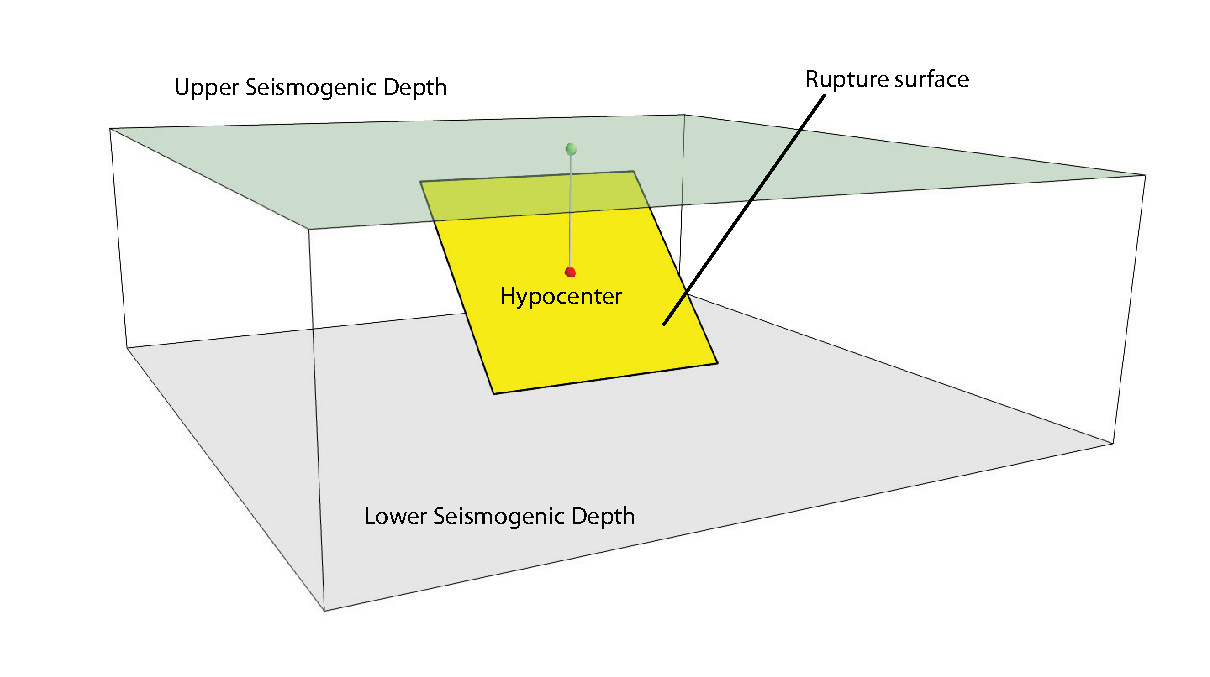
\includegraphics[width=10cm]{figures/hazard/single_rupture.pdf}
\caption{Single rupture}
\label{fig:single_rupture}
\end{figure}

The point source is the elemental source type adopted in the OpenQuake-engine
for modelling distributed seismicity. The OpenQuake-engine always performs
calculations considering finite ruptures, even in the case of point sources.

These are the basic assumptions used to generate ruptures with point sources:

\begin{itemize}

    \item Ruptures have a rectangular shape

    \item Rupture hypocenter is located in the middle of the rupture

    \item Ruptures are limited at the top and at the bottom by two planes
    parallel to the topographic surface and placed at two characteristic
    depths named upper and lower seismogenic depths, respectively (see
    Figure~\ref{fig:single_rupture})

\end{itemize}

\paragraph{Source data}

For the definition of a point source the following parameters are required
(Figure~\ref{fig:single_rupture} shows some of the parameters described
below, together with an example of the surface of a generated rupture):

\begin{itemize}

    \item The coordinates of the point (i.e. longitude and latitude) [decimal
    degrees]

    \item The upper and lower seismogenic depths [km]

    \item One \gls{mfd}

    \item One magnitude-scaling relationship

    \item The rupture aspect ratio

    \item A distribution of nodal planes i.e. one (or several) instances
    of the following set of parameters:

    \begin{itemize}
        \item \gls{strike} [degrees]
        \item \gls{dip} [degrees]
        \item \gls{rake} [degrees]
    \end{itemize}

\item A magnitude independent depth distribution of hypocenters [km].

\end{itemize}

Figure~\ref{fig:point_source_multiple_ruptures} shows ruptures generated by a
point source for a range of magnitudes. Each rupture is centered on the
single hypocentral position admitted by this point source. Ruptures are
created by conserving the area computed using the specified magnitude-area
scaling relatioship and the corresponding value of magnitude.

\begin{figure}[ht!]
\centering
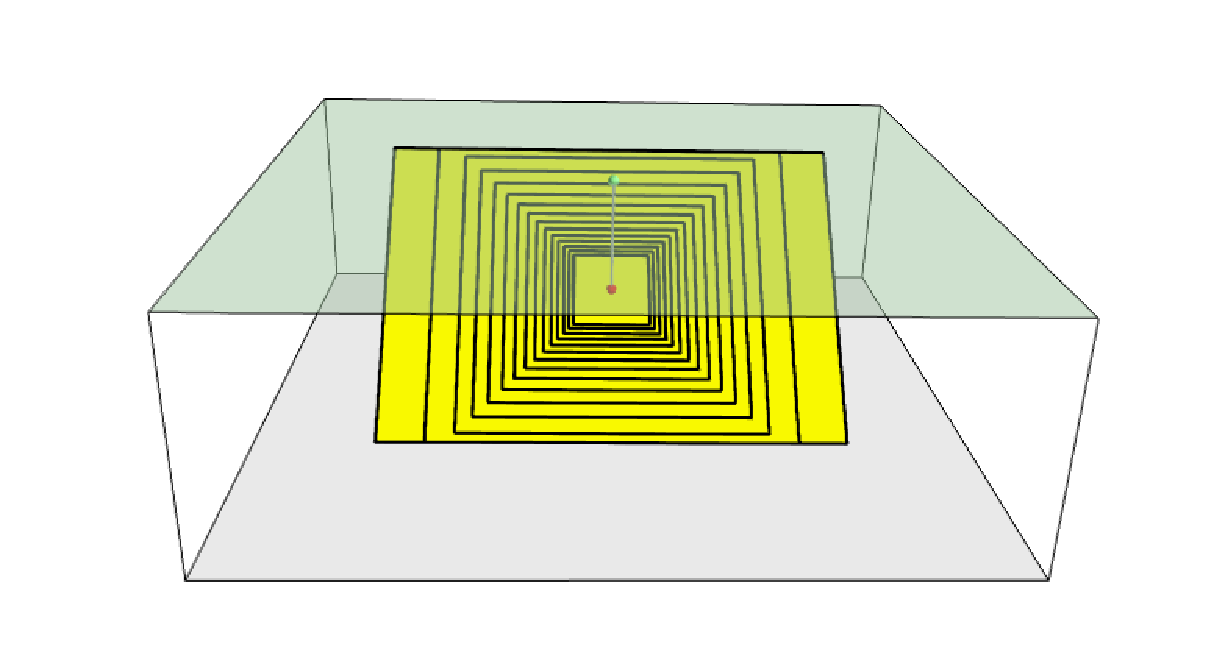
\includegraphics[width=10cm]{figures/hazard/point_source_multiple_ruptures.pdf}
\caption{Point source with multiple ruptures. Note the change in the aspect
ratio once the rupture width fills the entire seismogenic layer.}
\label{fig:point_source_multiple_ruptures}
\end{figure}

Below we provide the excerpt of an .xml file used to describe the properties
of a point source:

\begin{Verbatim}[frame=single, commandchars=\\\{\}, fontsize=\footnotesize,
    numbers=left, numbersep=2pt]
<pointSource id="1" name="point" tectonicRegion="Stable Continental Crust">
    \textcolor{red}{<pointGeometry>}
        \textcolor{red}{<gml:Point>}
            \textcolor{red}{<gml:pos>-122.0 38.0</gml:pos>}
        \textcolor{red}{</gml:Point>}
        \textcolor{red}{<upperSeismoDepth>0.0</upperSeismoDepth>}
        \textcolor{red}{<lowerSeismoDepth>10.0</lowerSeismoDepth>}
    \textcolor{red}{</pointGeometry>}
    <magScaleRel>WC1994</magScaleRel>
    <ruptAspectRatio>0.5</ruptAspectRatio>
    \textcolor{blue}{<truncGutenbergRichterMFD aValue="-3.5" bValue="1.0" minMag="5.0" }
			\textcolor{blue}{maxMag="6.5" />}
    \textcolor{green}{<nodalPlaneDist>}
        \textcolor{green}{<nodalPlane probability="0.3" strike="0.0" dip="90.0" rake="0.0" />}
        \textcolor{green}{<nodalPlane probability="0.7" strike="90.0" dip="45.0" rake="90.0" />}
    \textcolor{green}{</nodalPlaneDist>}
    \textcolor{magenta}{<hypoDepthDist>}
        \textcolor{magenta}{<hypoDepth probability="0.5" depth="4.0" />}
        \textcolor{magenta}{<hypoDepth probability="0.5" depth="8.0" />}
    \textcolor{magenta}{</hypoDepthDist>}
</pointSource>
\end{Verbatim}
\label{page:point_source_nrml}

The red part shows the the parameters used to describe the geometry of the
point source, the blue part is the description of the magnitude-frequency
distribution, the green text shows the nodal plane distribution and the text
in magenta illustrates the hypocentral depth distribution.

The text in black describes the parameters needed to generate the ruptures
such as the \gls{msr} and the aspect ratio.

Note that in this example, ruptures occur on two possible nodal planes and
two hypocentral depths. Figure~\ref{fig:point_source_ruptures} shows the
ruptures generated by the point source specified above.

\begin{figure}[!ht]
\centering
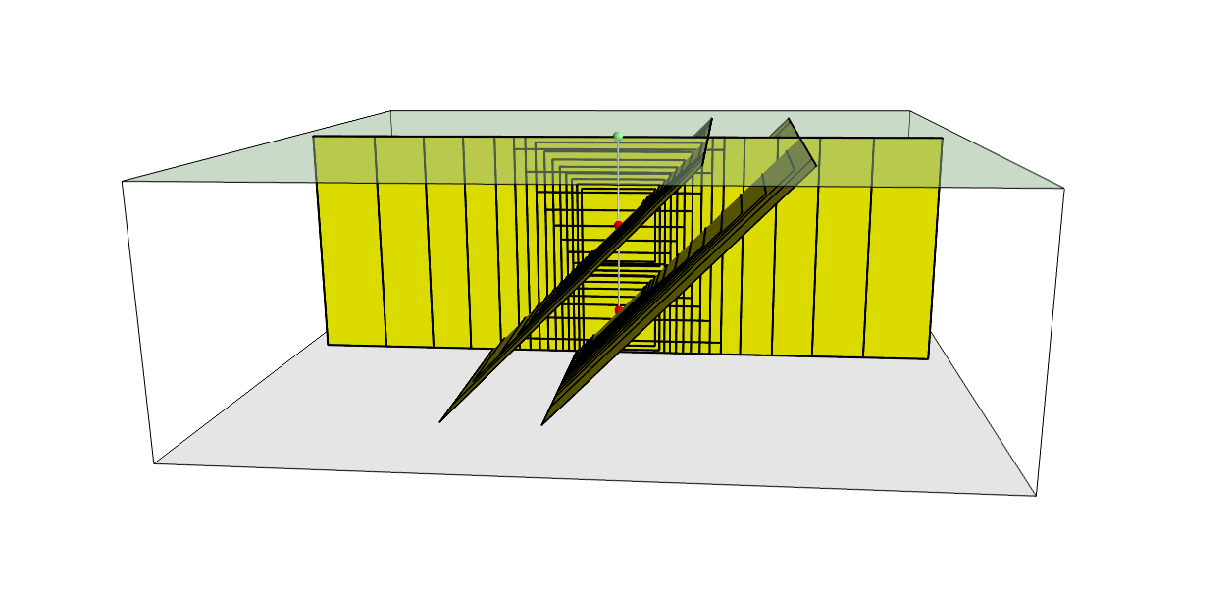
\includegraphics[width=10cm]{figures/hazard/pointsrc_2strike_2hypodep.pdf}
\caption{Ruptures produced by the source created using the information 
in the example .xml file described at page~\pageref{page:point_source_nrml}.}
\label{fig:point_source_ruptures}
\end{figure}



\subsubsection{Grid sources}
\label{subsubsec:grid_sources}
\index{Source type!grid}
\index{Grid source|see{Source type}}

A \gls{gridsource} is simply a collection of point sources distributed over a
regular grid (usually equally spaced in longitude and latitude).

In \gls{psha} a grid source can be considered a model alternative to area
sources, since they both model distributed seismicity.

Grid sources are generally used to reproduce more faithfully the spatial
pattern of seismicity depicted by the earthquakes occurred in the past; in
some models (e.g. \citet{petersen2008}) only events of low and intermediate
magnitudes are considered.

Grid sources are generally computed using seismicity smoothing algorithms
\citep[][amongst many others]{frankel1995,woo1996}.

The use of smoothing algorithms to produce grid sources brings some
advantages compared to area sources, since (1) it removes most of the
unavoidable degree of subjectivity due to the definition of the geometries of
the area sources and (2) it produces a spatial pattern of seismicity that is
usually closer to what observed in the reality. Nevertheless, in many cases
smoothing algorithms require an a-priori definition of some setup parameters
that expose the calculation to a certain degree of partiality.

Grid sources are modeled in \gls{acr:oqe} simply as a set of point sources; in
other words, a grid source is just a long list of point sources specified as
described in the previous section (see page
\pageref{subsubsec:point_sources}).



\subsubsection{Area sources}
\label{subsubsec:area_sources}
\index{Source type!area}
\index{Area source|see{Source type}}

Area sources are usually adopted to describe the seismicity occurring over
wide areas where the identification and characterization - i.e. the
unambiguous definition of position, geometry and seismicity occurrence
parameters - of single fault structures is difficult.

From a computation standpoint, area sources are comparable to grid sources
since they are both represented in the engine by a list of point sources.

The \gls{acr:oqe} using the source data parameters (see below) creates an
equally spaced in distance grid of point sources where each point has the same
seismicity occurrence properties (i.e. rate of events generated).

Below we provide a brief description of the parameters necessary to completely
describe an area source.

\paragraph{Source data}

\begin{itemize}

    \item A polygon defining the external border of the area (i.e. a list of
    Longitude-Latitude [degrees] tuples) The current version of the OQ-engine doesn't
    support the definition of internal borders.

    \item The upper and lower seismogenic depths [km]

    \item One gls{mfd}

    \item One gls{msr}

    \item The rupture aspect ratio

    \item A distribution of nodal planes i.e. one (or several) instances of
    the following set of parameters

    \begin{itemize}
        \item \gls{strike} [degrees]
        \item \gls{dip} [degrees]
        \item \gls{rake} [degrees]
    \end{itemize}

    \item A magnitude independent depth distribution of hypocenters [km].

\end{itemize}

Below we provide the exerpt of an .xml file used to describe the properties of
an area source:

\begin{Verbatim}[frame=single, commandchars=\\\{\}, fontsize=\footnotesize,
numbers=left, numbersep=2pt]
<areaSource id="1" name="Quito" tectonicRegion="Active Shallow Crust">
  <areaGeometry>
    <gml:Polygon>
      <gml:exterior>
        <gml:LinearRing>
          <gml:posList>
            -122.5 37.5
            -121.5 37.5
            -121.5 38.5
            -122.5 38.5
          </gml:posList>
        </gml:LinearRing>
      </gml:exterior>
    </gml:Polygon>
    <upperSeismoDepth>0.0</upperSeismoDepth>
    <lowerSeismoDepth>10.0</lowerSeismoDepth>
  </areaGeometry>
  <magScaleRel>PeerMSR</magScaleRel>
  <ruptAspectRatio>1.5</ruptAspectRatio>
  <incrementalMFD minMag="6.55" binWidth="0.1">
    <occurRates>0.0010614989 8.8291627E-4 7.3437777E-4 6.108288E-4
       5.080653E-4</occurRates>
  </incrementalMFD>
  <nodalPlaneDist>
  <nodalPlane probability="0.3" strike="0.0" dip="90.0" rake="0.0"/>
    <nodalPlane probability="0.7" strike="90.0" dip="45.0" rake="90.0"/>
  </nodalPlaneDist>
  <hypoDepthDist>
    <hypoDepth probability="0.5" depth="4.0" />
    <hypoDepth probability="0.5" depth="8.0" />
  </hypoDepthDist>
</areaSource>
\end{Verbatim}

The red text describes the parameters used to describe the geometry of the
area source; the blue part is the description of the magnitude-frequency
distribution; the green text displays the nodal plane distribution; and the
text in magenta illustrates the hypocentral depth distribution.

The text in gray describes the parameters required to generate the ruptures
such as the \gls{msr} and the aspect ratio.

The ruptures generated by the area source described in the example above are
controlled by two nodal planes and have hypocenters at localized at two
distinct depths.

\subsection{Fault sources with floating ruptures}
Fault sources in the \gls{acr:oqe} are classified according to the method
adopted to distribute ruptures over the fault surface. Two options are
currently supported:

\begin{itemize}

    \item With the first option, ruptures with a surface lower than the
    whole fault surface are floated so as to cover as much as possible
    homogeneously the fault surface. This model is compatible with all the
    supported magnitude-frequency distributions.

    \item With the second option, ruptures always fill the entire fault
    surface. This model is compatible with magnitude-frequency
    distributions similar to a characteristic model (\`{a} la
    \cite{schwartz1984}).

\end{itemize}

In this subsection we discuss the different fault source types that
support floating ruptures. In the next subsection we will illustrate the fault
typology available to model a characteristic rupturing behaviour.



\subsubsection{Simple faults}
\label{desc_simple_fault}
\index{Source type!fault!simple geometry}
\index{Simple fault|see{Source type}}

Simple Faults are the most common source type used to model shallow faults;
the ``simple'' adjective relates to the geometry description of the source
which is obtained by projecting the fault trace (i.e. a polyline) along a
characteristic dip direction.

The parameters used to create an instance of this source type are described
in the following paragraph.

\paragraph{Source data}

\begin{itemize}

    \item A \gls{faulttrace} (usually a polyline). It is a list of
    longitude-latitude tuples [degrees]

    \item A \gls{frequencymagnitudedistribution}

    \item A \gls{msr}

    \item A representative value of the dip angle (specified following
    the Aki-Richards convention; see \citet{aki2002}) [degrees]

    \item Rake angle (specified following the Aki-Richards convention;
    see \citet{aki2002}) [degrees]

    \item Upper and lower depth values limiting the seismogenic interval [km]

\end{itemize}

For near-fault probabilistic seismic hazard analysis, two additional
parameters are needed for characterising seismic sources:

\begin{itemize}

    \item A hypocentre list. It is a list of the possible hypocentral
    positions, and the corresponding weights, e.g., alongStrike="0.25"
    downDip="0.25" weight="0.25". Each hypocentral position is defined in
    relative terms using as a reference the upper left corner of the rupture
    and by specifying the fraction of rupture length and rupture width.

    \item A slip list. It is a list of the possible rupture slip directions
    [degrees], and their corresponding weights. The angle describing each slip
    direction is measured counterclockwise using the fault strike direction as
    reference.

\end{itemize}

In near-fault PSHA calculations, the hypocentre list and the slip list are
mandatory. The weights in each list must always sum to one. The available GMPE
which currently supports the near-fault directivity PSHA calculation in OQ-
engine is the ChiouYoungs2014NearFaultEffect GMPE developed  by
\citet{chiou2014update} (associated with an \texttt{Active Shallow Crust}
tectonic region type).

Below we provide two examples of simple fault source files. The first is an
excerpt of an xml file used to describe the properties of a simple fault
source and the second example shows the excerpt of an xml file used to
describe the properties of a simple fault source that can be used to perform a
PSHA calculation taking into account directivity effects.

\begin{Verbatim}[frame=single, commandchars=\\\{\}, fontsize=\footnotesize,
numbers=left, numbersep=2pt]
<areaSource id="1" name="Quito" tectonicRegion="Active Shallow Crust">
    \textcolor{red}{<areaGeometry>}
        \textcolor{red}{<gml:Polygon>}
            \textcolor{red}{<gml:exterior>}
                \textcolor{red}{<gml:LinearRing>}
                    \textcolor{red}{<gml:posList>}
                    \textcolor{red}{-122.5 37.5}
                    \textcolor{red}{-121.5 37.5}
                    \textcolor{red}{-121.5 38.5}
                    \textcolor{red}{-122.5 38.5}
                    \textcolor{red}{</gml:posList>}
                    \textcolor{red}{</gml:LinearRing>}
            \textcolor{red}{</gml:exterior>}
        \textcolor{red}{</gml:Polygon>}
        \textcolor{red}{<upperSeismoDepth>0.0</upperSeismoDepth>}
        \textcolor{red}{<lowerSeismoDepth>10.0</lowerSeismoDepth>}
        \textcolor{red}{</areaGeometry>}
    \textcolor{gray}{<magScaleRel>PeerMSR</magScaleRel>}
    \textcolor{gray}{<ruptAspectRatio>1.5</ruptAspectRatio>}
    \textcolor{blue}{<incrementalMFD minMag="6.55" binWidth="0.1">}
        \textcolor{blue}{<occurRates>0.0010614989 8.8291627E-4 7.3437777E-4 6.108288E-4}
            \textcolor{blue}{5.080653E-4</occurRates>}
    \textcolor{blue}{</incrementalMFD>}
    \textcolor{green}{<nodalPlaneDist>}
        \textcolor{green}{<nodalPlane probability="0.3" strike="0.0" dip="90.0" rake="0.0"/>}
        \textcolor{green}{<nodalPlane probability="0.7" strike="90.0" dip="45.0" rake="90.0"/>}
    \textcolor{green}{</nodalPlaneDist>}
    \textcolor{magenta}{<hypoDepthDist>}
        \textcolor{magenta}{<hypoDepth probability="0.5" depth="4.0" />}
        \textcolor{magenta}{<hypoDepth probability="0.5" depth="8.0" />}
    \textcolor{magenta}{</hypoDepthDist>}
</areaSource>
\end{Verbatim}
\label{example_incremental_mfd}

Below is an excerpt of a simple fault source xml file for near-fault
directivity PSHA calculations:

\begin{Verbatim}[frame=single, commandchars=\\\{\}, fontsize=\footnotesize,
    numbers=left, numbersep=2pt]
<simpleFaultSource id="1" name="Mount Diablo Thrust"
        tectonicRegion="Active Shallow Crust">
    \textcolor{red}{<simpleFaultGeometry>}
        \textcolor{red}{<gml:LineString>}
            \textcolor{red}{<gml:posList>}
                \textcolor{red}{-121.82290 37.73010}
                \textcolor{red}{-122.03880 37.87710}
            \textcolor{red}{</gml:posList>}
        \textcolor{red}{</gml:LineString>}
        \textcolor{red}{<dip>45.0</dip>}
        \textcolor{red}{<upperSeismoDepth>10.0</upperSeismoDepth>}
        \textcolor{red}{<lowerSeismoDepth>20.0</lowerSeismoDepth>}
    \textcolor{red}{</simpleFaultGeometry>}
    \textcolor{gray}{<magScaleRel>WC1994</magScaleRel>}
    \textcolor{gray}{<ruptAspectRatio>1.5</ruptAspectRatio>}
    \textcolor{blue}{<incrementalMFD minMag="5.0" binWidth="0.1">}
        \textcolor{blue}{<occurRates>0.0010614989 8.8291627E-4 7.3437777E-4 6.108288E-4 }
                \textcolor{blue}{5.080653E-4</occurRates>}
    \textcolor{blue}{</incrementalMFD>}
    \textcolor{green}{<rake>30.0</rake>}
    \textcolor{gray}{<hypoList>}
        \textcolor{gray}{<hypo alongStrike="0.25" downDip="0.25" weight="0.25"/>}
        \textcolor{gray}{<hypo alongStrike="0.25" downDip="0.75" weight="0.25"/>}
        \textcolor{gray}{<hypo alongStrike="0.75" downDip="0.25" weight="0.25"/>}
        \textcolor{gray}{<hypo alongStrike="0.75" downDip="0.75" weight="0.25"/>}
    \textcolor{gray}{</hypoList>}
    \textcolor{gray}{<slipList>}
        \textcolor{gray}{<slip weight="0.333"> 0.0 </slip>}
        \textcolor{gray}{<slip weight="0.333"> 45.0 </slip>}
        \textcolor{gray}{<slip weight="0.334"> 90.0 </slip>}
    \textcolor{gray}{</slipList>}
</simpleFaultSource>
\end{Verbatim}

As with the previous examples, the red text highlights the parameters used to
specify the source geometry, the parameters in green describe the rupture
mechanism, the text in blue describes the magnitude-frequency distribution and
the gray text describes the rupture properties.



\subsubsection{Complex faults}
\label{desc_complex_fault}
\index{Source type!fault!complex geometry}
\index{Complex fault|see{Source type}}

A complex fault differs from simple fault just by the way the geometry of the
fault surface is defined and the fault surface is later created. The input
parameters used to describe complex faults are, for the most part, the same
used to describe the simple fault typology.

In case of complex faults the dip angle is not requested while the fault trace
is substituted by two fault edges limiting at the top and bottom the fault
surface. Additional curves lying over the fault surface can be specified to
complement and refine the description of the fault surface geometry.

Usually, we use complex faults to model intraplate megathrust faults such as
the big subduction structures active in the Pacific (Sumatra, South America,
Japan) but this source typology can be used also to create - for example -
listric fault sources with a realistic geometry.

\begin{Verbatim}[frame=single, commandchars=\\\{\}, fontsize=\footnotesize,
    numbers=left, numbersep=2pt]
<complexFaultSource id="1" name="Cascadia Megathrust"
        tectonicRegion="Subduction Interface">
\textcolor{red}{    <complexFaultGeometry>}
\textcolor{red}{        <faultTopEdge>}
\textcolor{red}{            <gml:LineString>}
\textcolor{red}{                <gml:posList>}
\textcolor{red}{                    -124.704  40.363  0.5493260E+01}
\textcolor{red}{                    -124.977  41.214  0.4988560E+01}
\textcolor{red}{                    -125.140  42.096  0.4897340E+01}
\textcolor{red}{                </gml:posList>}
\textcolor{red}{            </gml:LineString>}
\textcolor{red}{        </faultTopEdge>}
\textcolor{red}{        <intermediateEdge>}
\textcolor{red}{            <gml:LineString>}
\textcolor{red}{                <gml:posList>}
\textcolor{red}{                    -124.704  40.363  0.5593260E+01}
\textcolor{red}{                    -124.977  41.214  0.5088560E+01}
\textcolor{red}{                    -125.140  42.096  0.4997340E+01}
\textcolor{red}{                </gml:posList>}
\textcolor{red}{            </gml:LineString>}
\textcolor{red}{        </intermediateEdge>}
\textcolor{red}{        <intermediateEdge>}
\textcolor{red}{            <gml:LineString>}
\textcolor{red}{                <gml:posList>}
\textcolor{red}{                    -124.704  40.363  0.5693260E+01}
\textcolor{red}{                    -124.977  41.214  0.5188560E+01}
\textcolor{red}{                    -125.140  42.096  0.5097340E+01}
\textcolor{red}{                </gml:posList>}
\textcolor{red}{            </gml:LineString>}
\textcolor{red}{        </intermediateEdge>}
\textcolor{red}{        <faultBottomEdge>}
\textcolor{red}{            <gml:LineString>}
\textcolor{red}{                <gml:posList>}
\textcolor{red}{                    -123.829  40.347  0.2038490E+02}
\textcolor{red}{                    -124.137  41.218  0.1741390E+02}
\textcolor{red}{                    -124.252  42.115  0.1752740E+02}
\textcolor{red}{                </gml:posList>}
\textcolor{red}{            </gml:LineString>}
\textcolor{red}{        </faultBottomEdge>}
\textcolor{red}{    </complexFaultGeometry>}
    \textcolor{gray}{<magScaleRel>WC1994</magScaleRel>}
    \textcolor{gray}{<ruptAspectRatio>1.5</ruptAspectRatio>}
\textcolor{blue}{   <truncGutenbergRichterMFD aValue="-3.5" bValue="1.0" minMag="5.0" }
\textcolor{blue}{           maxMag="6.5" />}
\textcolor{green}{   <rake>30.0</rake>}
</complexFaultSource>
\end{Verbatim}

As with the previous examples, the red text highlights the parameters used to
specify the source geometry, the parameters in green describe the rupture
mechanism, the text in blue describes the magnitude-frequency distribution and
the gray text describes the rupture properties.


\subsection{Fault sources without floating ruptures}
\subsubsection{Characteristic faults}
\index{Source type!fault!characteristic}
\index{Characteristic fault|see{Source type}}

The charactercistic fault source is a particular typology of fault created
with the assumption that its ruptures will always cover the entire fault
surface.

In this case, the fault surface can be represented either as a
\gls{simplefaultsource} surface or as a \gls{complexfaultsource} surface or as
a combination of rectangular ruptures as represented in
Figure~\ref{fig:char_fault_source}.

\begin{figure}[!ht]
\centering
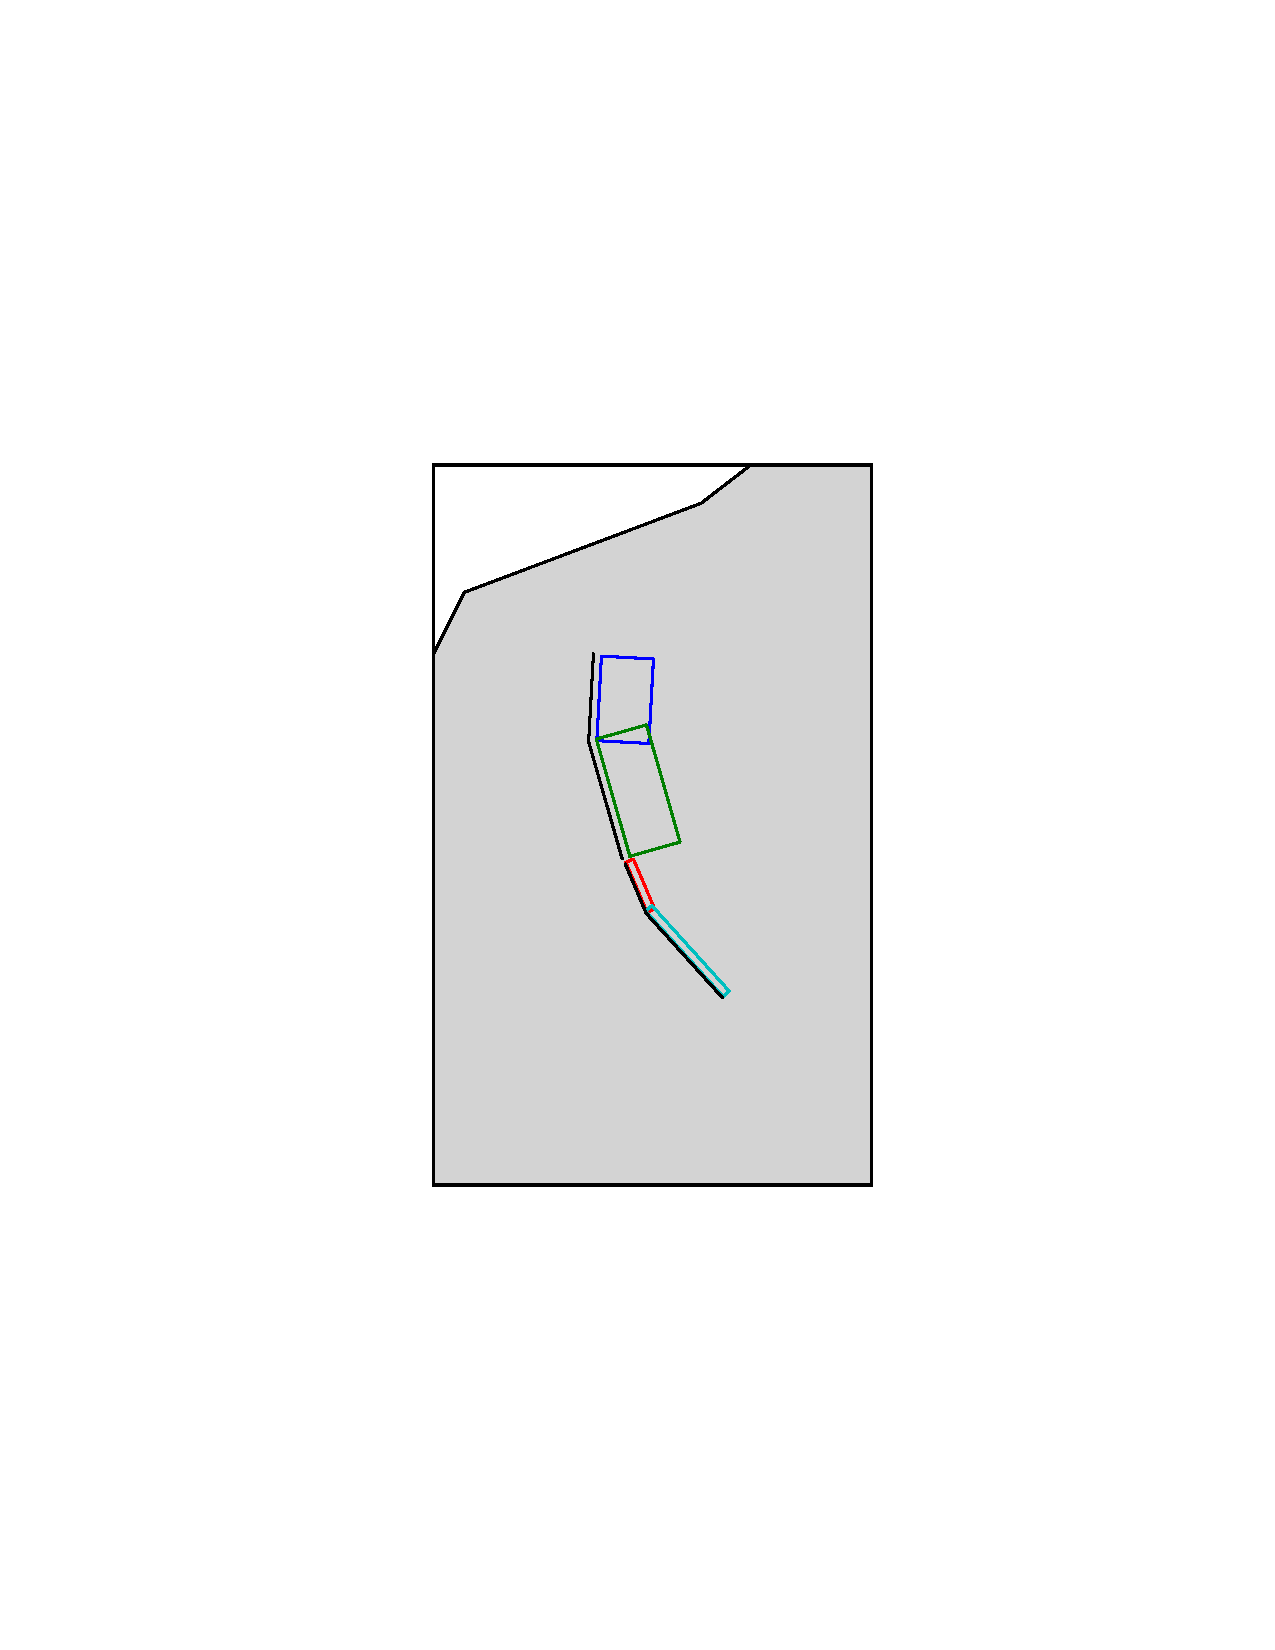
\includegraphics[width=15cm]{figures/hazard/multi_surface.pdf}
\caption{Geometry of a multi-segmented characteristic fault composed of four
         rectangular ruptures as modelled in OpenQuake.}
\label{fig:char_fault_source}
\end{figure}

\paragraph{Source data}

\begin{itemize}

    \item The characteristic rupture surface is defined through one of the
    following options:

        \begin{itemize}

            \item A list of rectangular ruptures

            \item A \gls{simplefaultsource} geometry

            \item A \gls{complexfaultsource} geometry

        \end{itemize}

    \item A \gls{frequencymagnitudedistribution}.

    \item Rake angle (specified following the Aki-Richards convention; see
          \citet{aki2002}).

    \item Upper and lower depth values limiting the seismogenic interval.

\end{itemize}



\section{Magnitude-frequency distributions}
\label{sec:mfd_list}
\subsection{Supported magnitude-frequency distributions}
\label{sec:mfd}
The magnitude-frequency distributions currently supported by the 
\gls{acr:oqe} are the following: 
\begin{description}
    \item[A discrete incremental magnitude-frequency distribution] \hfill \\
    It's the simplest distribution offered. It's defined by a 
    minimum value of magnitude (representing the mid point of the first
    bin) and the bin width. The distribution itself is simply a 
    sequence of floats describing the annual number of events for 
    different bins (centered on increasing values of magnitude). 
    Below we show an example of the xml used to describe an incremental 
    \glspl{acr:mfd} for a seismic source input of a \gls{acr:ssim}.
\begin{Verbatim}[frame=single, commandchars=\\\{\}, fontsize=\footnotesize]
<incrementalMFD minMag="5.05" binWidth="0.1">
    <occurRates>0.15 0.08 0.05 0.03 0.015</occurRates>
</incrementalMFD>
\end{Verbatim}
    This is the magnitude-frequency distribution obtained with the above
    settings:
% ..............................................................................
% . . . . . . . . . . . . . . . . . . . . . . . . . . . . . . . . . . . > Figure
\begin{figure}[!ht]
\centering
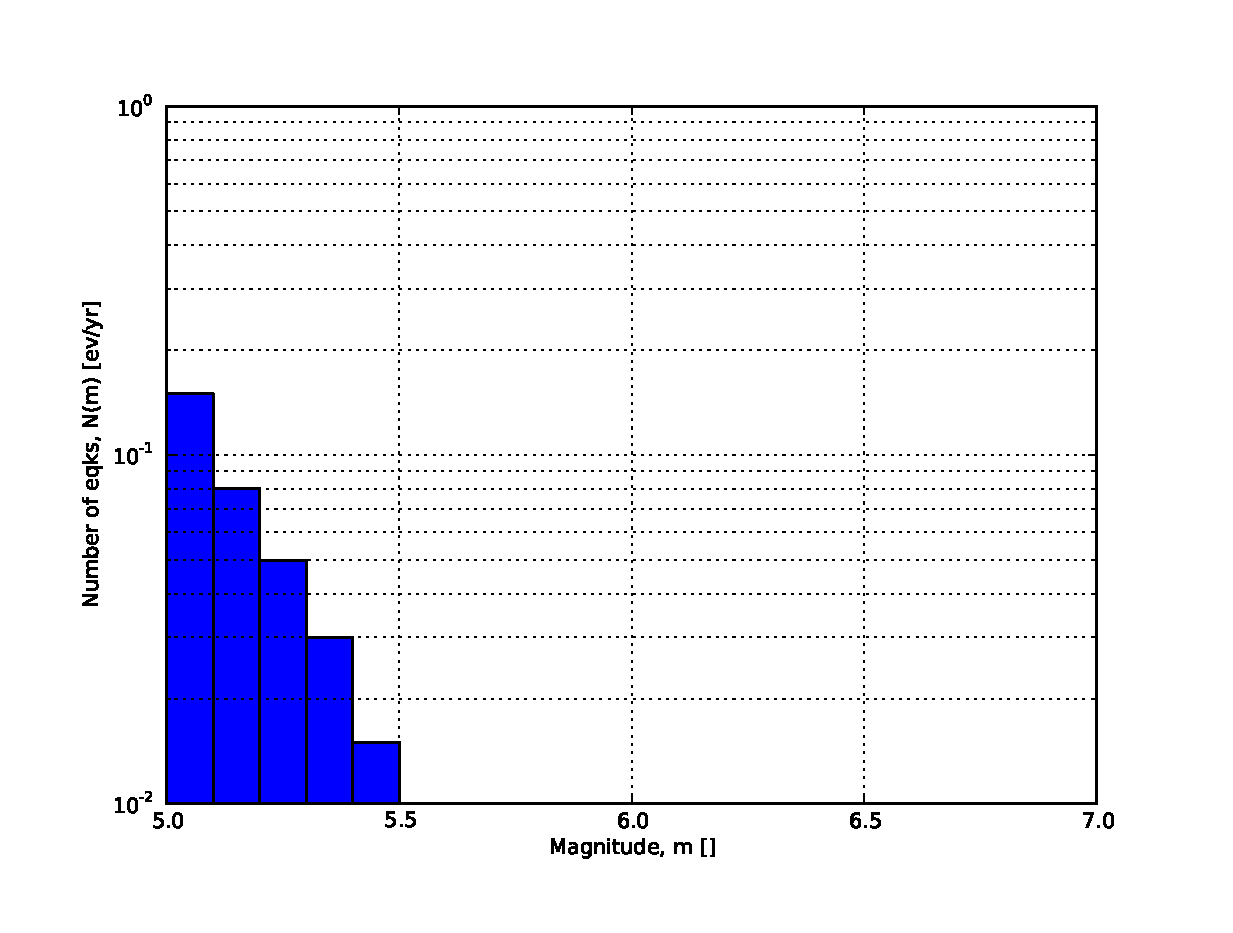
\includegraphics[width=12cm]{./figures/hazard/ed_mfd.eps}
\caption{Incremental magnitude-frequency distribution.}
\label{fig:evenly_discretized_mfd}
\end{figure}
% . . . . . . . . . . . . . . . . . . . . . . . . . . . . . . . . . . . < Figure
% ..............................................................................
%
\item[A double truncated Gutenberg-Richter distribution] \hfill \\
    This distribution is de\-scribed by means of a minimum \texttt{minMag}
    and maximum magnitude \texttt{maxMag} and by the $a$ and $b$ values 
    of the Gutenberg-Richter relationship. The synthax of the xml is 
    rather compact as shown below
\begin{Verbatim}[frame=single, commandchars=\\\{\}, fontsize=\footnotesize]
<truncGutenbergRichterMFD aValue="5.0" bValue="1.0" minMag="5.0" 
        maxMag="6.0"/>
\end{Verbatim}
    This is the magnitude-frequency distribution obtained using the 
    parameters of the considered example:
% ..............................................................................
% . . . . . . . . . . . . . . . . . . . . . . . . . . . . . . . . . . . > Figure
\begin{figure}[!ht]
\centering
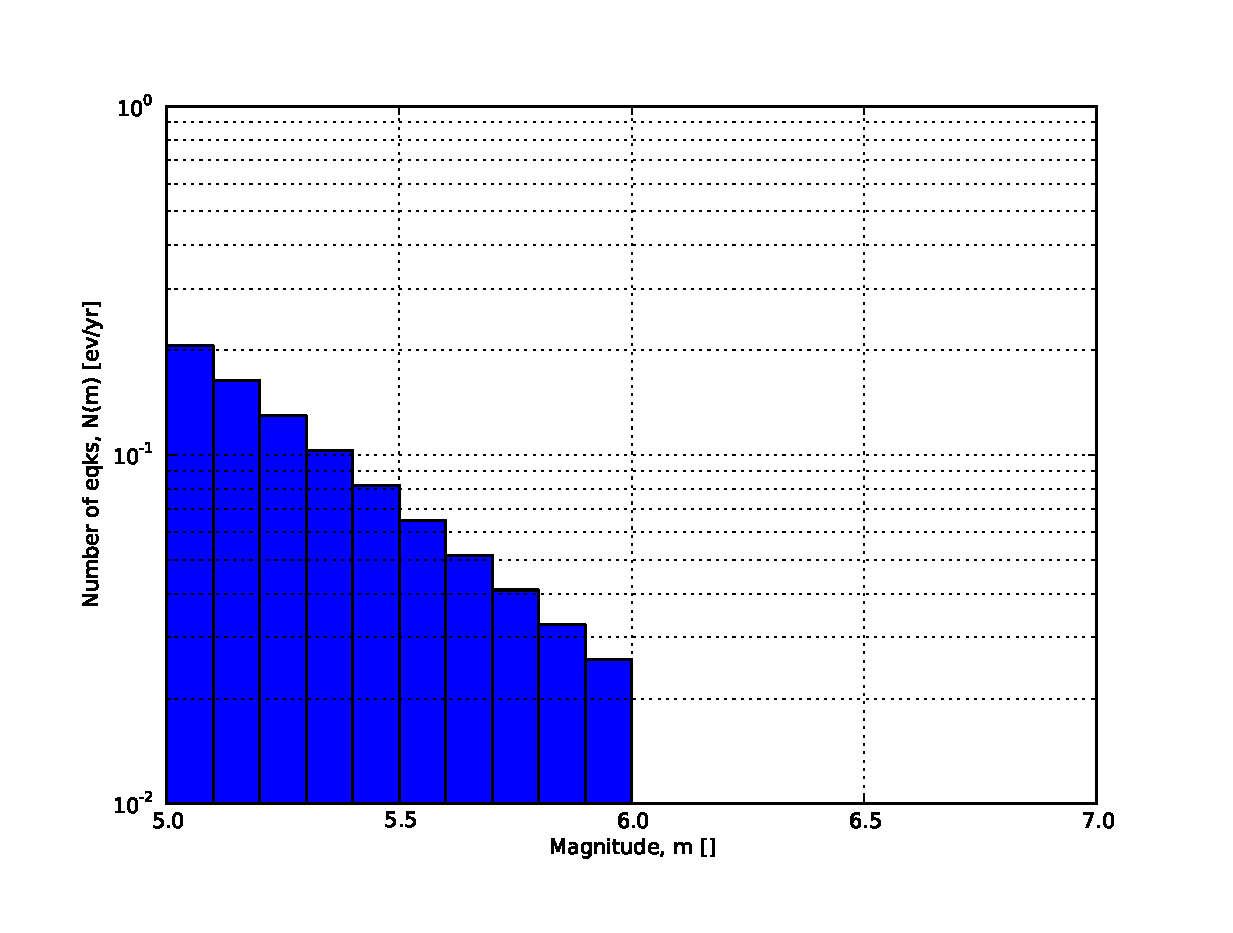
\includegraphics[width=12cm]{./figures/hazard/dt_mfd.eps}
\caption{Double truncated Gutenberg-Richter magnitude-frequency distribution.}
\label{fig:dt_gr_mfd}
\end{figure}
% . . . . . . . . . . . . . . . . . . . . . . . . . . . . . . . . . . . < Figure
% ..............................................................................
%
\item[Characteristic earthquake model (\`{a} la \cite{youngs1985})]
    The 
\begin{Verbatim}[frame=single, commandchars=\\\{\}, fontsize=\footnotesize]
    AA
\end{Verbatim}
% ..............................................................................
% . . . . . . . . . . . . . . . . . . . . . . . . . . . . . . . . . . . > Figure
\begin{figure}[!ht]
\centering
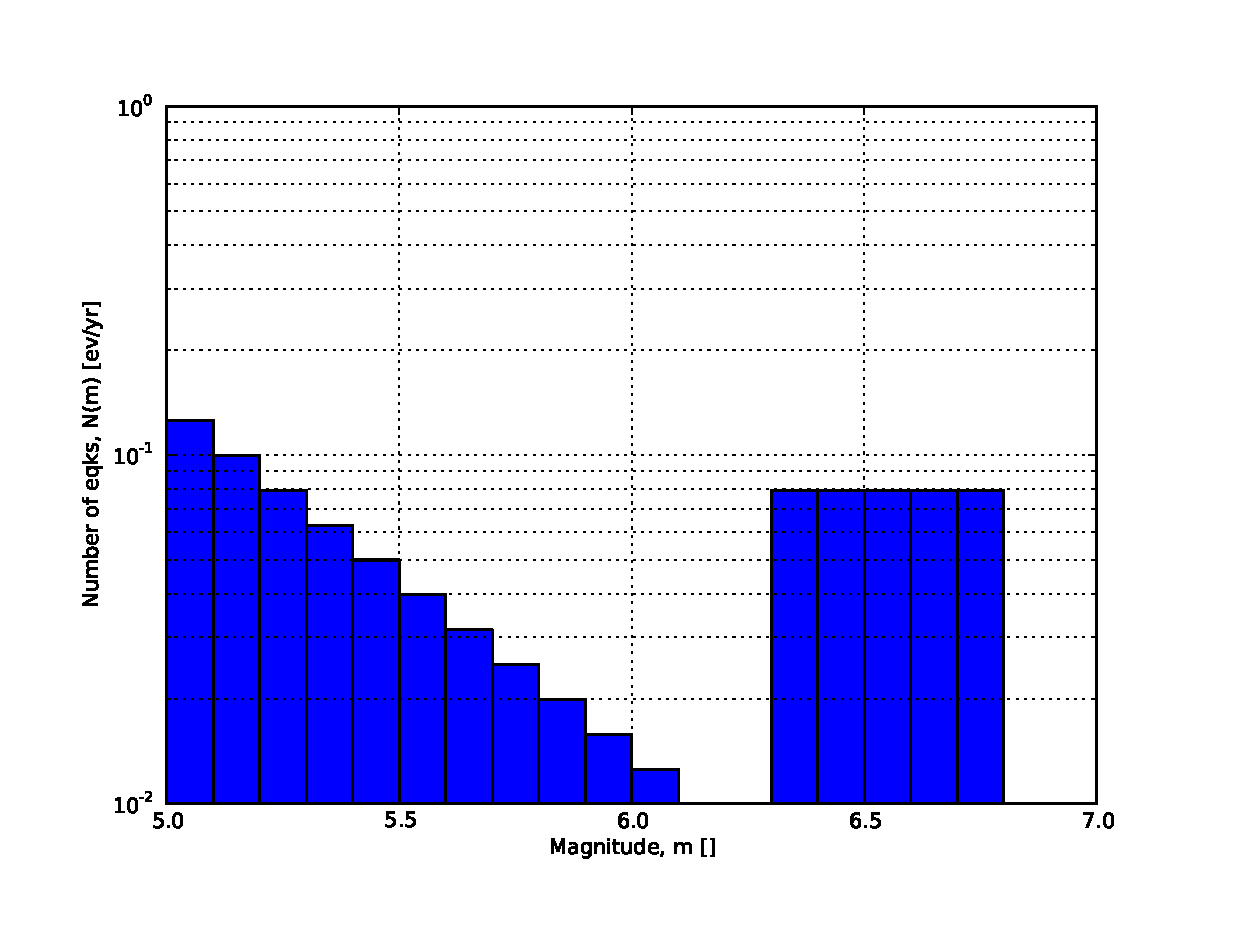
\includegraphics[width=12cm]{./figures/hazard/yc_mfd.eps}
\caption{\cite{youngs1985} magnitude-frequency distribution.}
\label{fig:yc_gr_mfd}
\end{figure}
% . . . . . . . . . . . . . . . . . . . . . . . . . . . . . . . . . . . < Figure
% ..............................................................................

\end{description}


\section{Magnitude-scaling relationships}
\label{sec:msr_list}
\subsection{Relationships for shallow earthquakes in active tectonic regions}

We provide below a list of the magnitude-area scaling relationships
implemented in the \gls{acr:hazlib}:

\begin{itemize}

    \item \cite{wells1994} - One of the most well known magnitude scaling
	relationships, based on a global database of historical earthquake
	ruptures. The implemented relationship is the one linking magnitude to
	rupture area.

\end{itemize}


%\subsection{Magnitude-scaling relationships for subduction earthquakes}
%\begin{itemize}
%    \item
%\end{itemize}
%
%\subsection{Magnitude-scaling relationships stable continental regions}
%\begin{itemize}
%    \item
%\end{itemize}
%
%\subsection{Ground motion prediction equations for volcanic areas}
%\begin{itemize}
%    \item
%\end{itemize}

\section{Calculation workflows}
\index{OpenQuake-engine!Hazard calculation workflows}
\label{sec:hazard_calculators}
The hazard component of the OpenQuake-engine can compute seismic hazard using
various approaches. Three types of analysis are currently supported:

\begin{itemize}

	\item \textit{Classical Probabilistic Seismic Hazard Analysis (PSHA)},
	allowing calculation of hazard curves and hazard maps following the
	classical integration procedure (\cite{cornell1968}, \citet{mcguire1976})
	as formulated by \cite{field2003}.

	\item \textit{Event-Based Probabilistic Seismic Hazard Analysis},
	allowing calculation of ground-motion fields from stochastic event sets.
	Traditional results - such as hazard curves - can be obtained by post-
	processing the set of computed ground-motion fields.

	\item \textit{\gls{acr:ssha}}, allowing the calculation of ground
	motion fields from a single earthquake rupture scenario taking into
	account ground-motion aleatory variability.

\end{itemize}

Each workflow has a modular structure, so that intermediate results can be
exported and analyzed. Each calculator can be extended independently of the
others so that additional calculation options and methodologies can be easily
introduced, without affecting the overall calculation workflow.



\subsection{Classical Probabilistic Seismic Hazard Analysis}
\index{OpenQuake-engine!Hazard calculation workflows!Classical PSHA}
\label{subsec:classical_psha}
Input data for the classical \gls{acr:psha} consist of a PSHA input model
provided together with calculation settings.

The main calculators used to perform this analysis are the following:

\begin{enumerate}

	\item \emph{Logic Tree Processor}

	The Logic Tree Processor (LTP) takes as an input the \gls{acr:psha} Input
	Model and creates a Seismic Source Model. The LTP uses the information in
	the Initial Seismic Source Models and the Seismic Source Logic Tree to
	create a Seismic Source Input Model (i.e. a model describing geometry and
	activity rates of each source without any epistemic uncertainty).

	Following a procedure similar to the one just described the Logic Tree
	Processor creates a Ground Motion model (i.e. a data structure that
	associates to each tectonic region considered in the calculation a
	\gls{acr:gmpe}).

	\item \emph{Earthquake Rupture Forecast Calculator}

	The produced Seismic Source Input Model becomes an input information for
	the Earthquake Rupture Forecast (ERF) calculator which creates a list
	earthquake ruptures admitted by the source model, each one characterized
	by a probability of occurrence over a specified time span.

	\item \emph{Classical PSHA Calculator}

	The classical PSHA calculator uses the ERF and the Ground Motion model to
	compute hazard curves on each site specified in the calculation settings.

\end{enumerate}

\subsection{Event-Based Probabilistic Seismic Hazard Analysis}
\index{OpenQuake-engine!Hazard calculation workflows!Event-based PSHA}
\label{subsec:event_based_psha}
Input data for the Event-Based PSHA - as in the case of the Classical
\gls{acr:psha} calculator - consists of a PSHA Input Model and a set of
calculation settings.

The main calculators used to perform this analysis are:

\begin{enumerate}

	\item \emph{Logic Tree Processor}

	The Logic Tree Processor works in the same way described in  the
	description of the Classical \gls{acr:psha} workflow  (see
	Section~\ref{subsec:classical_psha} at
	page~\pageref{subsec:classical_psha}).

	\item \emph{Earthquake Rupture Forecast Calculator}

	The Earthquake Rupture Forecast Calculator was already  introduced in the
	description of the PSHA workflow (see Section~\ref{subsec:classical_psha}
	at page~\pageref{subsec:classical_psha}).

	\item \emph{Stochastic Event Set Calculator}

	The Stochastic Event Set Calculator generates a collection of stochastic
	event sets by sampling the ruptures contained in the ERF according to
	their probability of occurrence.

	A Stochastic Event Set (SES) thus represents a potential realisation of
	the seismicity (i.e. a list of ruptures) produced by the set of seismic
	sources considered in the analysis over the time span fixed for the
	calculation of hazard.

	\item \emph{Ground Motion Field Calculator}

	The Ground Motion Field Calculator computes for each event contained in a
	Stochastic Event Set a realization of the geographic distribution of the
	shaking by taking into account the aleatory uncertainties in the ground-
	motion model. Eventually, the Ground Motion Field calculator can consider
	the spatial correlation of the ground-motion during the generation of the
	\gls{acr:gmf}.

	\item \emph{Event-based PSHA Calculator}

	The event-based PSHA calculator takes a (large) set of ground-motion
	fields representative of the possible shaking scenarios that the
	investigated area can experience over a (long) time span and for each
	site computes the corresponding hazard curve.

	This procedure is computationally intensive and is not recommended for
	investigating the hazard over large areas.

\end{enumerate}

\subsection{Scenario based Seismic Hazard Analysis}
\index{OpenQuake-engine!Hazard calculation workflows!Scenario-based SHA}
\label{subsec:scenario_hazard}
In case of \gls{acr:ssha}, the input data consist of a single earthquake
rupture model and one or more ground-motion models. Using the Ground Motion Field Calculator, multiple realizations of ground shaking can be computed, each realization sampling the aleatory uncertainties in the ground-motion model. The main calculator used to perform this analysis is the \emph{Ground Motion Field Calculator}, which was already introduced during the description of the event based PSHA workflow (see Section~\ref{subsec:event_based_psha} at page~\pageref{subsec:event_based_psha}).

As the scenario calculator does not need to determine the probability of occurrence of the specific rupture, but only sufficient information to parameterise the location (as a three-dimensional surface), the magnitude and the style-of-faulting of the rupture, a more simplified NRML structure is needed. A \emph{rupture model} XML can be defined in the following formats:

\begin{enumerate}
    \item \emph{Simple Fault Rupture} - in which the geometry is defined by the trace of the fault rupture, the dip and the upper and lower seismogenic depths. An example is shown below:
\begin{minted}[firstline=1,firstnumber=1,fontsize=\footnotesize,frame=single,bgcolor=lightgray]{xml}
<?xml version='1.0' encoding='utf-8'?>
<nrml xmlns:gml="http://www.opengis.net/gml"
      xmlns="http://openquake.org/xmlns/nrml/0.5">
    <simpleFaultRupture>
        <magnitude>7.0</magnitude>
        <rake>90.0</rake>
        <hypocenter lat="0.0" lon="0.0" depth="10.0"/>
        <simpleFaultGeometry>
            <gml:LineString>
                <gml:posList>
                    0.0 -0.3
                    0.0  0.3
                </gml:posList>
            </gml:LineString>
            <dip>90.0</dip>
            <upperSeismoDepth>2.0</upperSeismoDepth>
            <lowerSeismoDepth>20.0</lowerSeismoDepth>
        </simpleFaultGeometry>
    </simpleFaultRupture>
</nrml>
\end{minted}
\\
    \item \emph{Planar \& Multi-Planar Rupture} - in which the geometry is defined as a collection of one or more rectangular planes, each defined by four corners.

    \begin{minted}[firstline=1,firstnumber=1,fontsize=\footnotesize,frame=single,bgcolor=lightgray]{xml}
<?xml version='1.0' encoding='utf-8'?>
<nrml xmlns:gml="http://www.opengis.net/gml"
      xmlns="http://openquake.org/xmlns/nrml/0.5">
    <multiPlanesRupture>
        <magnitude>8.0</magnitude>
        <rake>90.0</rake>
        <hypocenter lat="-1.4" lon="1.1" depth="10.0"/>
            <planarSurface strike="90.0" dip="45.0">
                <topLeft lon="-0.8" lat="-2.3" depth="0.0" />
                <topRight lon="-0.4" lat="-2.3" depth="0.0" />
                <bottomLeft lon="-0.8" lat="-2.3890" depth="10.0" />
                <bottomRight lon="-0.4" lat="-2.3890" depth="10.0" />
            </planarSurface>
            <planarSurface strike="30.94744" dip="30.0">
                <topLeft lon="-0.42" lat="-2.3" depth="0.0" />
                <topRight lon="-0.29967" lat="-2.09945" depth="0.0" />
                <bottomLeft lon="-0.28629" lat="-2.38009" depth="10.0" />
                <bottomRight lon="-0.16598" lat="-2.17955" depth="10.0" />
            </planarSurface>
    </multiPlanesRupture>
</nrml> 
\end{minted}
\\
    \item \emph{Complex Fault Rupture} - in which the geometry is defined by the upper, lower and (if applicable) intermediate edges of the fault rupture.

\begin{minted}[firstline=1,firstnumber=1,fontsize=\footnotesize,frame=single,bgcolor=lightgray]{xml}
    <?xml version='1.0' encoding='utf-8'?>
<nrml xmlns:gml="http://www.opengis.net/gml"
      xmlns="http://openquake.org/xmlns/nrml/0.5">
    <complexFaultRupture>
        <magnitude>8.0</magnitude>
        <rake>90.0</rake>
        <hypocenter lat="-1.4" lon="1.1" depth="10.0"/>
        <complexFaultGeometry>
            <faultTopEdge>
                <gml:LineString>
                    <gml:posList>
                        0.6 -1.5 2.0
                        1.0 -1.3 5.0
                        1.5 -1.0 8.0
                    </gml:posList>
                </gml:LineString>
            </faultTopEdge>
            <intermediateEdge>
                <gml:LineString>
                    <gml:posList>
                        0.65 -1.55 4.0
                        1.1  -1.4  10.0
                        1.5  -1.2  20.0
                    </gml:posList>
                </gml:LineString>
            </intermediateEdge>
            <faultBottomEdge>
                <gml:LineString>
                    <gml:posList>
                        0.65 -1.7 8.0
                        1.1  -1.6 15.0
                        1.5  -1.7 35.0
                    </gml:posList>
                </gml:LineString>
            </faultBottomEdge>
        </complexFaultGeometry>
    </complexFaultRupture>
</nrml>
\end{minted}
\end{enumerate}


\cleardoublepage